% Standalone figures for WasmSentinel paper
% These can be included in the main document or compiled separately

% ============================================
% Figure 1: System Architecture (Detailed)
% ============================================
\begin{figure*}[t]
\centering
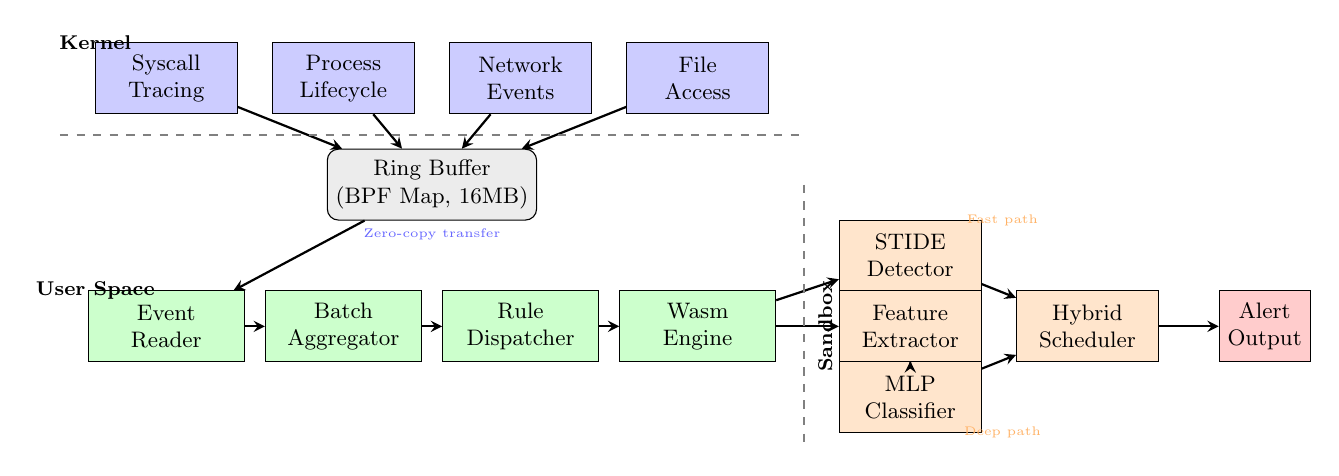
\begin{tikzpicture}[
    scale=0.9,
    transform shape,
    box/.style={rectangle, draw, minimum height=1cm, align=center, font=\small},
    ebpf/.style={box, fill=blue!20, minimum width=2cm},
    host/.style={box, fill=green!20, minimum width=2.2cm},
    wasm/.style={box, fill=orange!20, minimum width=2cm},
    data/.style={box, fill=gray!15, minimum width=2.5cm, rounded corners},
    arrow/.style={->, >=stealth, thick},
    label/.style={font=\footnotesize\bfseries}
]
    % Kernel Space
    \node[ebpf] (syscall) at (0,0) {Syscall\\Tracing};
    \node[ebpf] (sched) at (2.5,0) {Process\\Lifecycle};
    \node[ebpf] (net) at (5,0) {Network\\Events};
    \node[ebpf] (file) at (7.5,0) {File\\Access};

    \node[data] (ring) at (3.75,-1.5) {Ring Buffer\\(BPF Map, 16MB)};

    % User Space - Host
    \node[host] (reader) at (0,-3.5) {Event\\Reader};
    \node[host] (batcher) at (2.5,-3.5) {Batch\\Aggregator};
    \node[host] (dispatch) at (5,-3.5) {Rule\\Dispatcher};
    \node[host] (engine) at (7.5,-3.5) {Wasm\\Engine};

    % Wasm Sandbox
    \node[wasm] (stide) at (10.5,-2.5) {STIDE\\Detector};
    \node[wasm] (features) at (10.5,-3.5) {Feature\\Extractor};
    \node[wasm] (mlp) at (10.5,-4.5) {MLP\\Classifier};
    \node[wasm] (hybrid) at (13,-3.5) {Hybrid\\Scheduler};

    % Output
    \node[box, fill=red!20] (alert) at (15.5,-3.5) {Alert\\Output};

    % Arrows - Kernel
    \draw[arrow] (syscall) -- (ring);
    \draw[arrow] (sched) -- (ring);
    \draw[arrow] (net) -- (ring);
    \draw[arrow] (file) -- (ring);

    % Arrows - Host
    \draw[arrow] (ring) -- (reader);
    \draw[arrow] (reader) -- (batcher);
    \draw[arrow] (batcher) -- (dispatch);
    \draw[arrow] (dispatch) -- (engine);

    % Arrows - Wasm
    \draw[arrow] (engine) -- (stide);
    \draw[arrow] (engine) -- (features);
    \draw[arrow] (features) -- (mlp);
    \draw[arrow] (stide) -- (hybrid);
    \draw[arrow] (mlp) -- (hybrid);
    \draw[arrow] (hybrid) -- (alert);

    % Labels and boundaries
    \draw[dashed, thick, gray] (-1.5,-0.8) -- (9,-0.8);
    \node[label] at (-1, 0.5) {Kernel};
    \node[label] at (-1, -3) {User Space};

    \draw[dashed, thick, gray] (9,-1.5) -- (9,-5.2);
    \node[label, rotate=90] at (9.3, -3.5) {Sandbox};

    % Annotations
    \node[font=\tiny, text=blue!60] at (3.75,-2.2) {Zero-copy transfer};
    \node[font=\tiny, text=orange!60] at (11.8,-2) {Fast path};
    \node[font=\tiny, text=orange!60] at (11.8,-5) {Deep path};
\end{tikzpicture}
\caption{Detailed \textsc{WasmSentinel} architecture showing data flow from kernel eBPF programs through the host dispatcher to the Wasm-sandboxed detection modules.}
\label{fig:architecture-detailed}
\end{figure*}


% ============================================
% Figure 2: Latency Comparison Bar Chart
% ============================================
\begin{figure}[t]
\centering
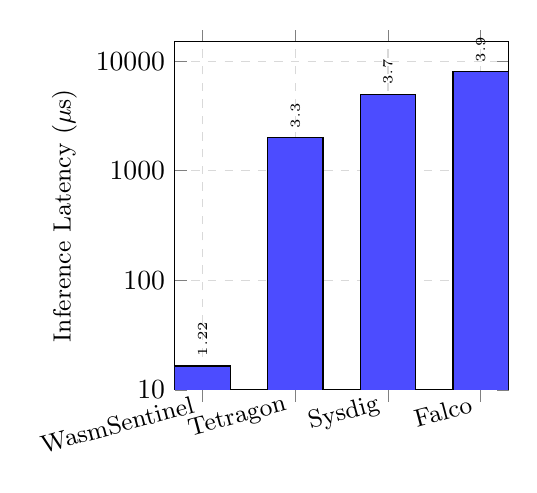
\begin{tikzpicture}
\begin{axis}[
    ybar,
    bar width=20pt,
    width=0.48\textwidth,
    height=6cm,
    ylabel={Inference Latency ($\mu$s)},
    ylabel style={font=\small},
    symbolic x coords={WasmSentinel, Tetragon, Sysdig, Falco},
    xtick=data,
    xticklabel style={font=\small, rotate=15, anchor=east},
    ymode=log,
    log basis y={10},
    ymin=10,
    ymax=15000,
    ytick={10, 100, 1000, 10000},
    yticklabels={10, 100, 1000, 10000},
    nodes near coords,
    every node near coord/.append style={font=\tiny, rotate=90, anchor=west},
    legend style={at={(0.98,0.98)}, anchor=north east, font=\tiny},
    grid=major,
    grid style={dashed, gray!30}
]
\addplot[fill=blue!70] coordinates {
    (WasmSentinel, 16.5)
    (Tetragon, 2000)
    (Sysdig, 5000)
    (Falco, 8000)
};
\end{axis}
\end{tikzpicture}
\caption{Inference latency comparison (log scale). \textsc{WasmSentinel} achieves 121--485$\times$ lower latency than existing systems.}
\label{fig:latency-comparison}
\end{figure}


% ============================================
% Figure 3: Throughput Comparison
% ============================================
\begin{figure}[t]
\centering
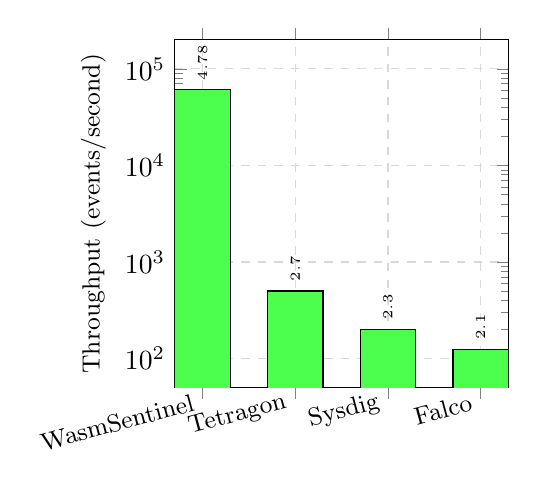
\begin{tikzpicture}
\begin{axis}[
    ybar,
    bar width=20pt,
    width=0.48\textwidth,
    height=6cm,
    ylabel={Throughput (events/second)},
    ylabel style={font=\small},
    symbolic x coords={WasmSentinel, Tetragon, Sysdig, Falco},
    xtick=data,
    xticklabel style={font=\small, rotate=15, anchor=east},
    ymode=log,
    log basis y={10},
    ymin=50,
    ymax=200000,
    nodes near coords,
    every node near coord/.append style={font=\tiny, rotate=90, anchor=west},
    grid=major,
    grid style={dashed, gray!30}
]
\addplot[fill=green!70] coordinates {
    (WasmSentinel, 60612)
    (Tetragon, 500)
    (Sysdig, 200)
    (Falco, 125)
};
\end{axis}
\end{tikzpicture}
\caption{Throughput comparison (log scale). \textsc{WasmSentinel} sustains over 60,000 events/second.}
\label{fig:throughput-comparison}
\end{figure}


% ============================================
% Figure 4: Memory Usage Comparison
% ============================================
\begin{figure}[t]
\centering
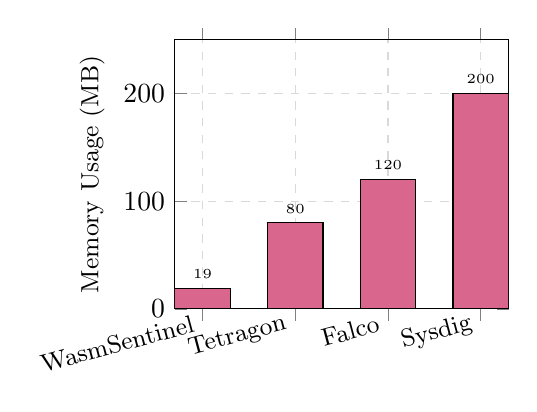
\begin{tikzpicture}
\begin{axis}[
    ybar,
    bar width=20pt,
    width=0.48\textwidth,
    height=5cm,
    ylabel={Memory Usage (MB)},
    ylabel style={font=\small},
    symbolic x coords={WasmSentinel, Tetragon, Falco, Sysdig},
    xtick=data,
    xticklabel style={font=\small, rotate=15, anchor=east},
    ymin=0,
    ymax=250,
    nodes near coords,
    every node near coord/.append style={font=\tiny},
    grid=major,
    grid style={dashed, gray!30}
]
\addplot[fill=purple!60] coordinates {
    (WasmSentinel, 19)
    (Tetragon, 80)
    (Falco, 120)
    (Sysdig, 200)
};
\end{axis}
\end{tikzpicture}
\caption{Memory footprint comparison. \textsc{WasmSentinel} uses 4--10$\times$ less memory.}
\label{fig:memory-comparison}
\end{figure}


% ============================================
% Figure 5: Architecture Search Results
% ============================================
\begin{figure}[t]
\centering
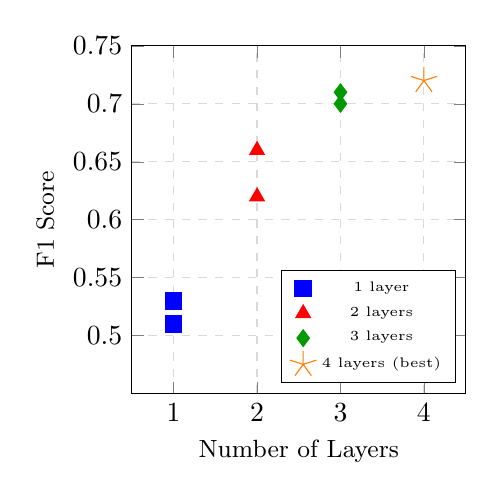
\begin{tikzpicture}
\begin{axis}[
    width=0.48\textwidth,
    height=6cm,
    xlabel={Number of Layers},
    ylabel={F1 Score},
    ylabel style={font=\small},
    xlabel style={font=\small},
    xmin=0.5, xmax=4.5,
    ymin=0.45, ymax=0.75,
    xtick={1,2,3,4},
    ytick={0.5, 0.55, 0.6, 0.65, 0.7, 0.75},
    legend pos=south east,
    legend style={font=\tiny},
    grid=major,
    grid style={dashed, gray!30},
    mark size=3pt
]
% Single layer models
\addplot[color=blue, mark=square*, only marks] coordinates {
    (1, 0.51)
    (1, 0.53)
    (1, 0.53)
};
% Two layer models
\addplot[color=red, mark=triangle*, only marks] coordinates {
    (2, 0.62)
    (2, 0.66)
};
% Three layer models
\addplot[color=green!60!black, mark=diamond*, only marks] coordinates {
    (3, 0.71)
    (3, 0.70)
};
% Four layer model
\addplot[color=orange, mark=star, only marks, mark size=5pt] coordinates {
    (4, 0.72)
};

\legend{1 layer, 2 layers, 3 layers, 4 layers (best)}
\end{axis}
\end{tikzpicture}
\caption{F1 score vs. network depth. Deeper networks achieve better accuracy, with diminishing returns beyond 4 layers.}
\label{fig:architecture-search}
\end{figure}


% ============================================
% Figure 6: Precision-Recall Trade-off
% ============================================
\begin{figure}[t]
\centering
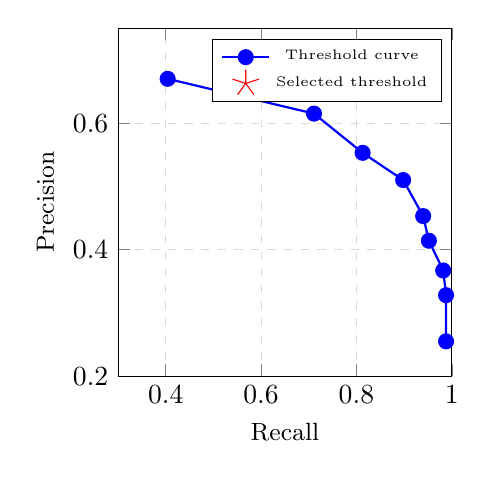
\begin{tikzpicture}
\begin{axis}[
    width=0.48\textwidth,
    height=6cm,
    xlabel={Recall},
    ylabel={Precision},
    ylabel style={font=\small},
    xlabel style={font=\small},
    xmin=0.3, xmax=1.0,
    ymin=0.2, ymax=0.75,
    legend pos=north east,
    legend style={font=\tiny},
    grid=major,
    grid style={dashed, gray!30},
    mark size=2.5pt
]
\addplot[color=blue, mark=*, thick] coordinates {
    (0.988, 0.255)
    (0.988, 0.328)
    (0.982, 0.367)
    (0.952, 0.414)
    (0.940, 0.453)
    (0.898, 0.510)
    (0.813, 0.553)
    (0.711, 0.615)
    (0.404, 0.670)
};
\addplot[color=red, mark=star, only marks, mark size=5pt] coordinates {
    (0.84, 0.67)
};
\node[font=\tiny] at (axis cs:0.78, 0.72) {Optimal};
\legend{Threshold curve, Selected threshold}
\end{axis}
\end{tikzpicture}
\caption{Precision-Recall curve showing the trade-off at different classification thresholds. The selected threshold (0.7) balances detection rate with false positive rate.}
\label{fig:pr-curve}
\end{figure}


% ============================================
% Figure 7: Hybrid Detection Flow
% ============================================
\begin{figure}[t]
\centering
\begin{tikzpicture}[
    scale=0.85,
    transform shape,
    box/.style={rectangle, draw, minimum height=0.8cm, align=center, font=\footnotesize, minimum width=1.5cm},
    decision/.style={diamond, draw, aspect=2.5, font=\footnotesize, inner sep=1pt},
    arrow/.style={->, >=stealth, thick}
]
    \node[box, fill=blue!15] (input) at (0,0) {Event\\Input};
    \node[box, fill=green!15] (stide) at (2.2,0) {STIDE\\Check};
    \node[decision, fill=yellow!15] (d1) at (4.5,0) {Anomaly?};
    \node[box, fill=green!15] (pass) at (4.5,-1.5) {Pass};
    \node[box, fill=orange!15] (feat) at (6.8,0) {Feature\\Extract};
    \node[box, fill=orange!15] (mlp) at (9,0) {MLP\\Inference};
    \node[decision, fill=yellow!15] (d2) at (11.3,0) {Threat?};
    \node[box, fill=red!20] (alert) at (11.3,1.5) {Alert};
    \node[box, fill=green!15] (benign) at (13.5,0) {Benign};

    \draw[arrow] (input) -- (stide);
    \draw[arrow] (stide) -- (d1);
    \draw[arrow] (d1) -- node[right, font=\tiny] {No} (pass);
    \draw[arrow] (d1) -- node[above, font=\tiny] {Yes} (feat);
    \draw[arrow] (feat) -- (mlp);
    \draw[arrow] (mlp) -- (d2);
    \draw[arrow] (d2) -- node[right, font=\tiny] {Yes} (alert);
    \draw[arrow] (d2) -- node[above, font=\tiny] {No} (benign);

    % Timing annotations
    \node[font=\tiny, text=gray] at (1.1, -0.6) {0.2$\mu$s};
    \node[font=\tiny, text=gray] at (5.6, -0.6) {3.1$\mu$s};
    \node[font=\tiny, text=gray] at (7.9, -0.6) {12.8$\mu$s};
\end{tikzpicture}
\caption{Hybrid detection flow with per-stage latency breakdown. STIDE filtering eliminates most benign events before expensive MLP inference.}
\label{fig:hybrid-flow-detailed}
\end{figure}


% ============================================
% Figure 8: Latency Distribution CDF
% ============================================
\begin{figure}[t]
\centering
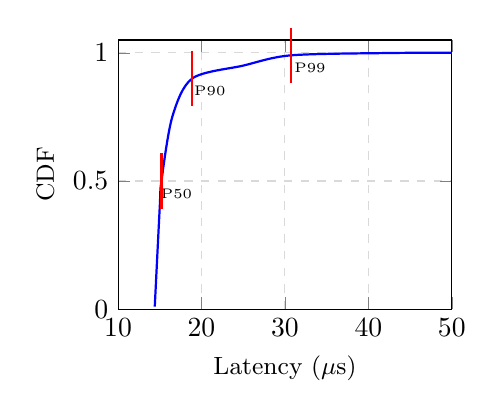
\begin{tikzpicture}
\begin{axis}[
    width=0.48\textwidth,
    height=5cm,
    xlabel={Latency ($\mu$s)},
    ylabel={CDF},
    ylabel style={font=\small},
    xlabel style={font=\small},
    xmin=10, xmax=50,
    ymin=0, ymax=1.05,
    legend pos=south east,
    legend style={font=\tiny},
    grid=major,
    grid style={dashed, gray!30}
]
\addplot[color=blue, thick, smooth] coordinates {
    (14.4, 0.01)
    (15.0, 0.40)
    (15.2, 0.50)
    (16.5, 0.75)
    (18.9, 0.90)
    (25.0, 0.95)
    (30.7, 0.99)
    (42.2, 0.999)
    (50, 1.0)
};
% P50, P90, P99 markers
\addplot[color=red, mark=|, only marks, mark size=10pt, thick] coordinates {
    (15.2, 0.50)
    (18.9, 0.90)
    (30.7, 0.99)
};
\node[font=\tiny] at (axis cs:17, 0.45) {P50};
\node[font=\tiny] at (axis cs:21, 0.85) {P90};
\node[font=\tiny] at (axis cs:33, 0.94) {P99};
\end{axis}
\end{tikzpicture}
\caption{Latency distribution CDF. Tail latency (P99=30.7$\mu$s) is only 2$\times$ the median, indicating consistent performance.}
\label{fig:latency-cdf}
\end{figure}
